\subsection{ADC Control} \label{subsec:ADC_CONTROL} 

The ADC control block is the controlling hardware for the two external LTC2311\cite{ADC_LTC2311} ADCs that are being used to sample the DUT voltage and current waveforms. The module should, when it sees a rising edge from another HDL block, start a sampling process through the ADCs, clock the data out of the ADCs, latch the data and set a data\_ready flag for the IV saver block to read the sampled data as shown on figure \refq{fig:7_2_8_ADCControlProcess}. This section will only concern itself with the timing of the ADC and the communication between the ADC and FPGA. The complete code for the ADC control module is quite long and can be seen in appendix \refq{App:ADCControlCode}. The code will be explained with diagrams as much as possible. 

\begin{figure}[H]
    \centering
    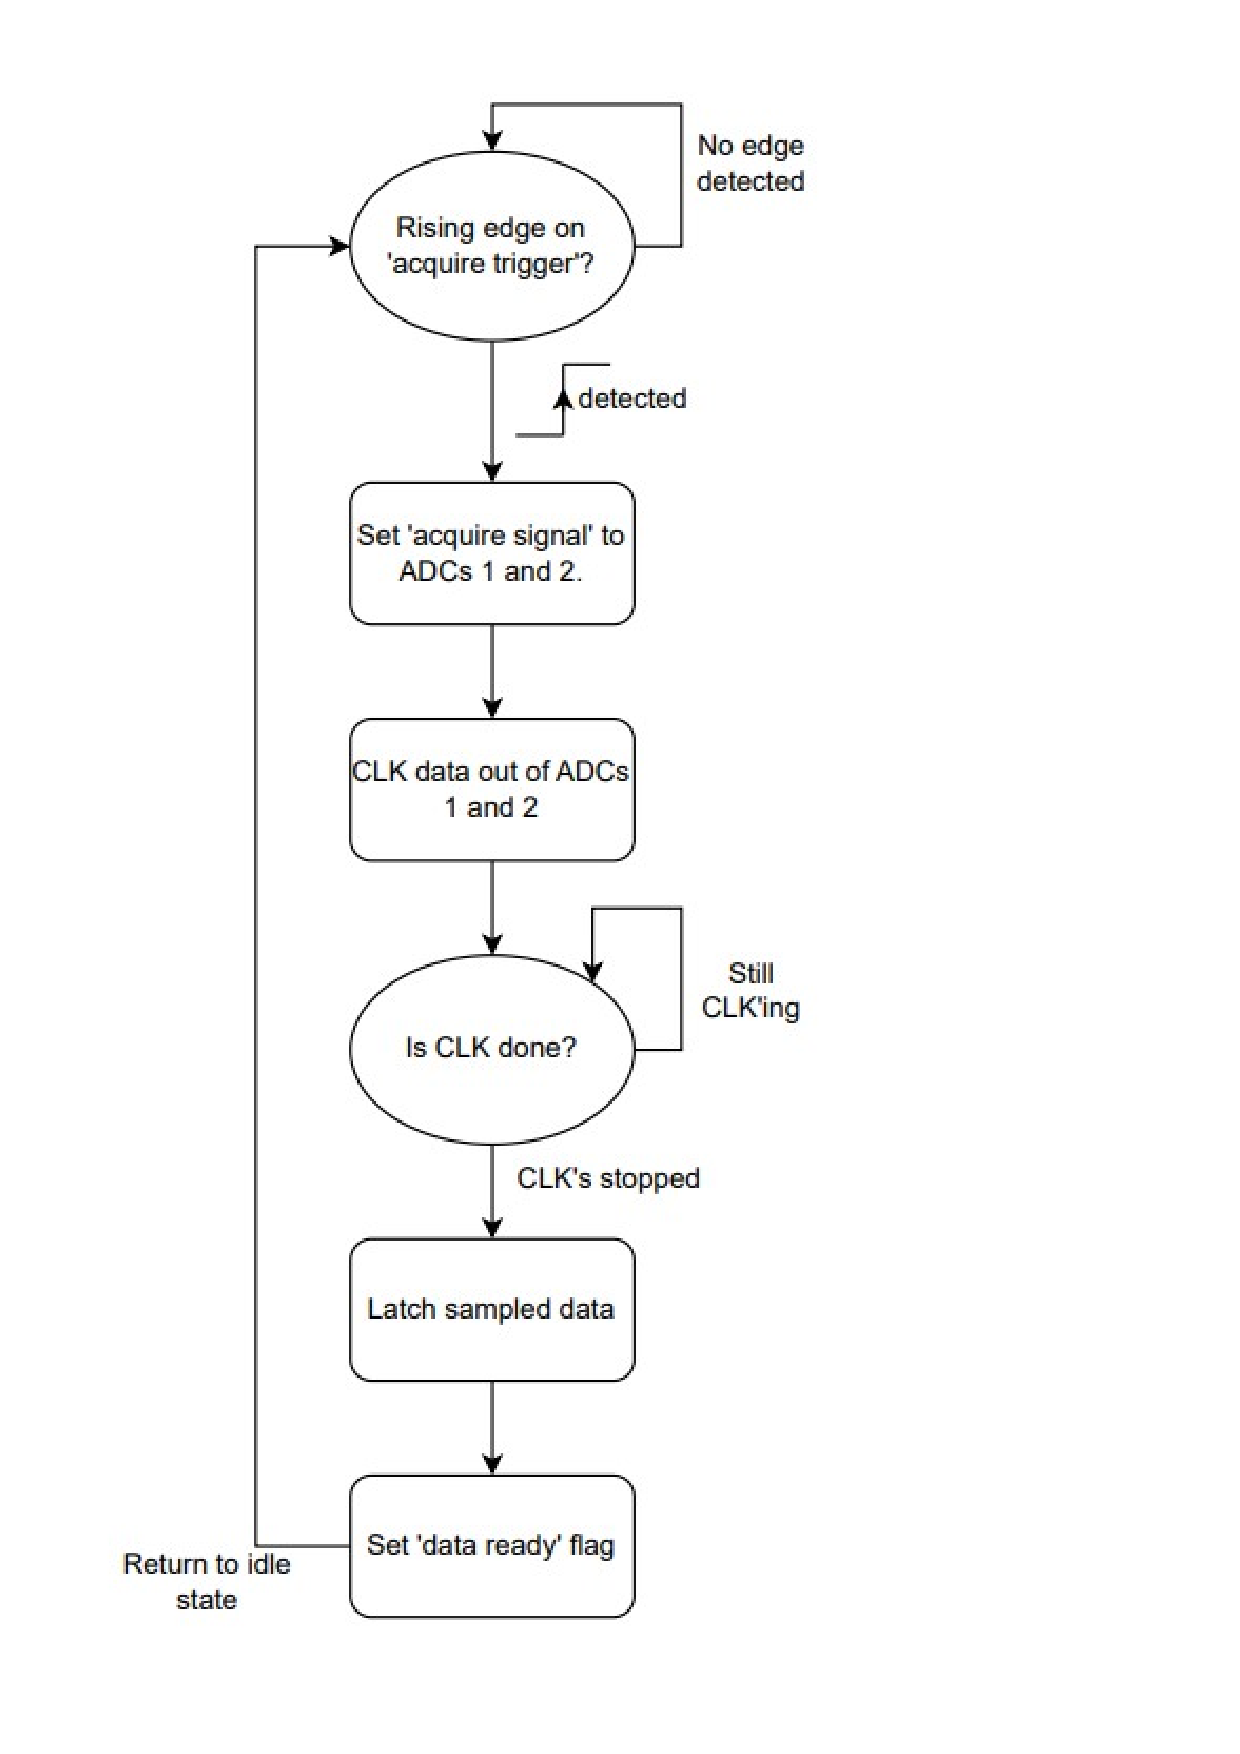
\includegraphics[clip, trim=0 0 0 0, width=0.6\textwidth]{Sections/7_SystemDesign/Figures/7_2_8_ADCControlOverallSignals_cropped.pdf}
    \caption{A process flow showing the overall function of the ADC control block. The block is 'triggered' on a rising edge of an input signal. The block will set an 'acquire' signal to the ADCs, which will start a sample and hold and AD-conversion process. The block will then clock out the sampled data, latch it, and let the next HDL block know that there is sample data ready for processing.}
    \label{fig:7_2_8_ADCControlProcess}
\end{figure}

In order to make the process flow in figure \refq{fig:7_2_8_ADCControlProcess} work the ADC control block must fulfill the timing requirements of the LTC2311 ADC. The timings can be seen on figure \refq{fig:7_2_8_LTC2311_TIMING} where some significant periods have been marked in red on the timing diagram. These will be explained in detail. 

\begin{figure}[H]
    \centering
    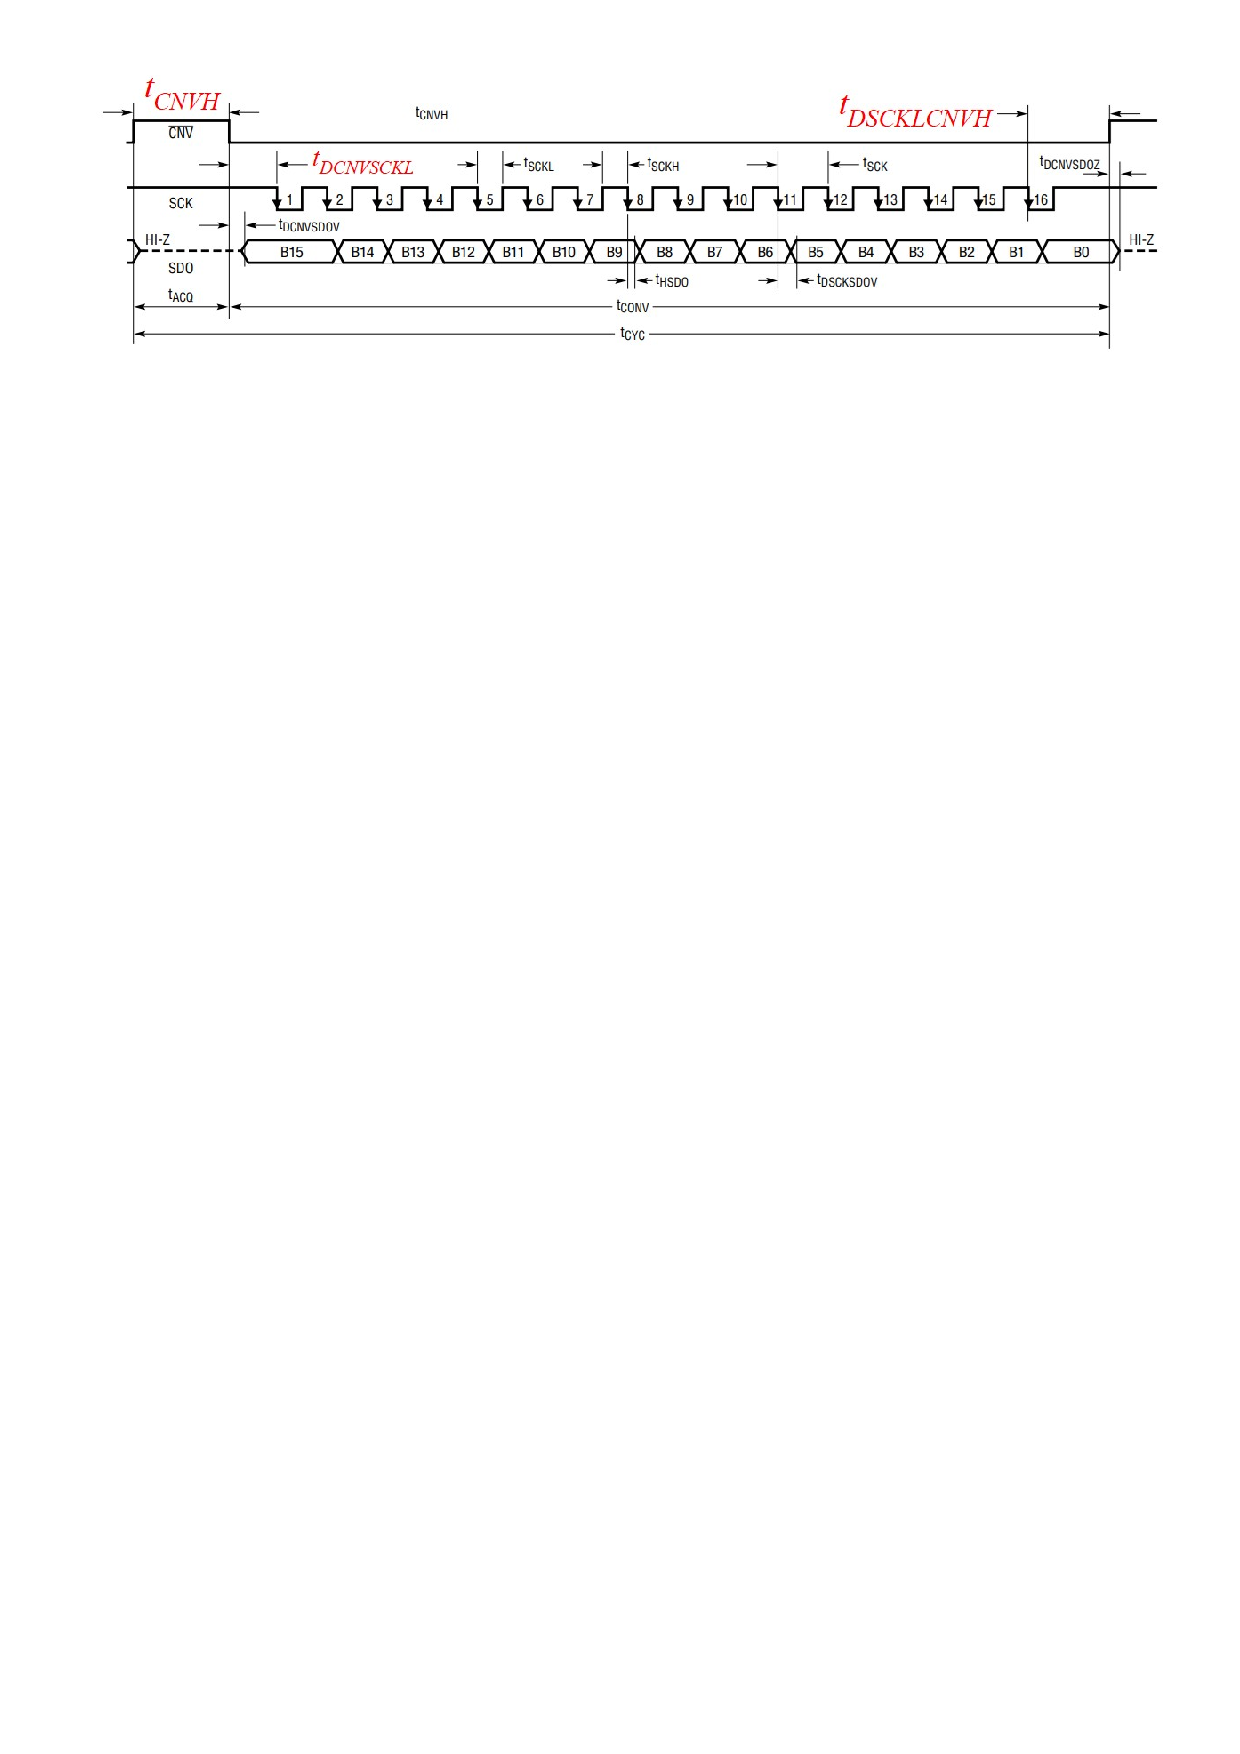
\includegraphics[clip, trim=0 675 0 0, width=1\textwidth]{Sections/7_SystemDesign/Figures/7_2_8_LTC2311_TIMING.pdf}
    \caption{A timing diagram of the communication between the LTC2311 ADC and an SPI master.}
    \label{fig:7_2_8_LTC2311_TIMING}
\end{figure}

The ADC starts an acquisition, i.e. samples the input, when the CNV signal transitions from '0' to '1' and digitizes the value during the $t_{CNVH}$ time. FIgure \refq{fig:7_2_8_LTC2311_TIMING} also lists this time as the acquisition time, $t_{ACQ}$. This time is important and the datasheet suggests $t_{CNVH} = 30 ns$ for a $5M sps$ sample rate. The ADC control block will be designed for a sample rate of $1 Msps$, even though the actual sample rate is expected to be much lower at this point. The main CLK in the sample control module is a \SIQ{200}{\mega\hertz} CLK with a period of $t_{clk} = 5 ns$, so a multiple of this clock period will be convenient for generating the CNV pulse.

The $t_{DCNVSCKL}$ period, marked in red on figure \refq{fig:7_2_8_LTC2311_TIMING}, is the time from a falling edge of CNV to the start of the SPI clock signal. Note how data is clocked out of the ADC on a falling edge of the SPI clock with the MSb being clocked out when the $t_{DCNVSCKL}$ time is passed. The minimum time is listed $t_{DCNVSCKL} = 9.5 ns$ (DCN) in the datasheet. Data is ready and can be clocked into the FPGA on a rising edge of the SPI clock signal as shown on the timing diagram. The $t_{DSCKLCNVH}$ period (DSC), is the minimum time that must pass from the LSb being clocked out of the ADC and until a new CNV pulse can be sent and a new acquisition started. The minimum time for the DSC period is listed as $t_{DSCKLCNVH} = 19.1 ns$.

Assuming $t_{CNV} = 35 ns$, $t_{DCN} = 10 ns$, $t_{DSC} = 20ns$ the SPI clock frequency can be found for a minimum sample rate of $1 MS/s$. The 'protocol' overhead is $t_p = 65 ns$ shown in \refq{eq:7_2_8_ProtocolOverhead}.
\begin{equation}\label{eq:7_2_8_ProtocolOverhead}
        t_{p} = t_{CNV} + t_{DCN} + t_{DSC} = 35e-9 + 10 e-9 + 20 e-9 = 65 e-9
\end{equation}
To get $f_{sample} = 1 MS/s$ with a sample period of $t_{sample} = 1e-6$ and a data packet size of 16 bits equation \refq{eq:7_2_8_SampleFrq} must be true.
\begin{equation}\label{eq:7_2_8_SampleFrq}
   \frac{1}{f_{SPICLK}} \cdot 16 + t_p = t_{sample}
\end{equation}
Using equation \refq{eq:7_2_8_SampleFrq} the sample frequency should, at minimum, be \SIQ{17.11}{\mega\hertz} as shown in equation \refq{eq:7_2_8_SampleFrq2}.
\begin{equation}\label{eq:7_2_8_SampleFrq2}
    f_{SPICLK} = -\frac{16}{t_{p} - t_{sample}} = -\frac{16}{65e-9 - 1e-6} = 17.11e6
 \end{equation}

The minimum SPI clock frequency should be \SIQ{17.11}{\mega\hertz}. This is not a multiple of \SIQ{5}{\nano\second} that the main clock of \SIQ{200}{\mega\hertz} works at. The SPI clock frequency will be set to $f_{SPICLK} = 20 MHz$ as this has a period of $t_{SPICLK} = 1/f_{SPICLK} = 50 ns$ and is a multiple of \SIQ{5}{\nano\second}.

 The ADC control module has been implemented as a state machine whose states will start and stop the various timing pulses required for the SPI communication with the ADCs. The FSM will start when it sees a rising edge of a trigger input signal as shown on figure \refq{fig:7_2_8_ADC_START_ACQ}.

\begin{figure}[H]
    \centering
    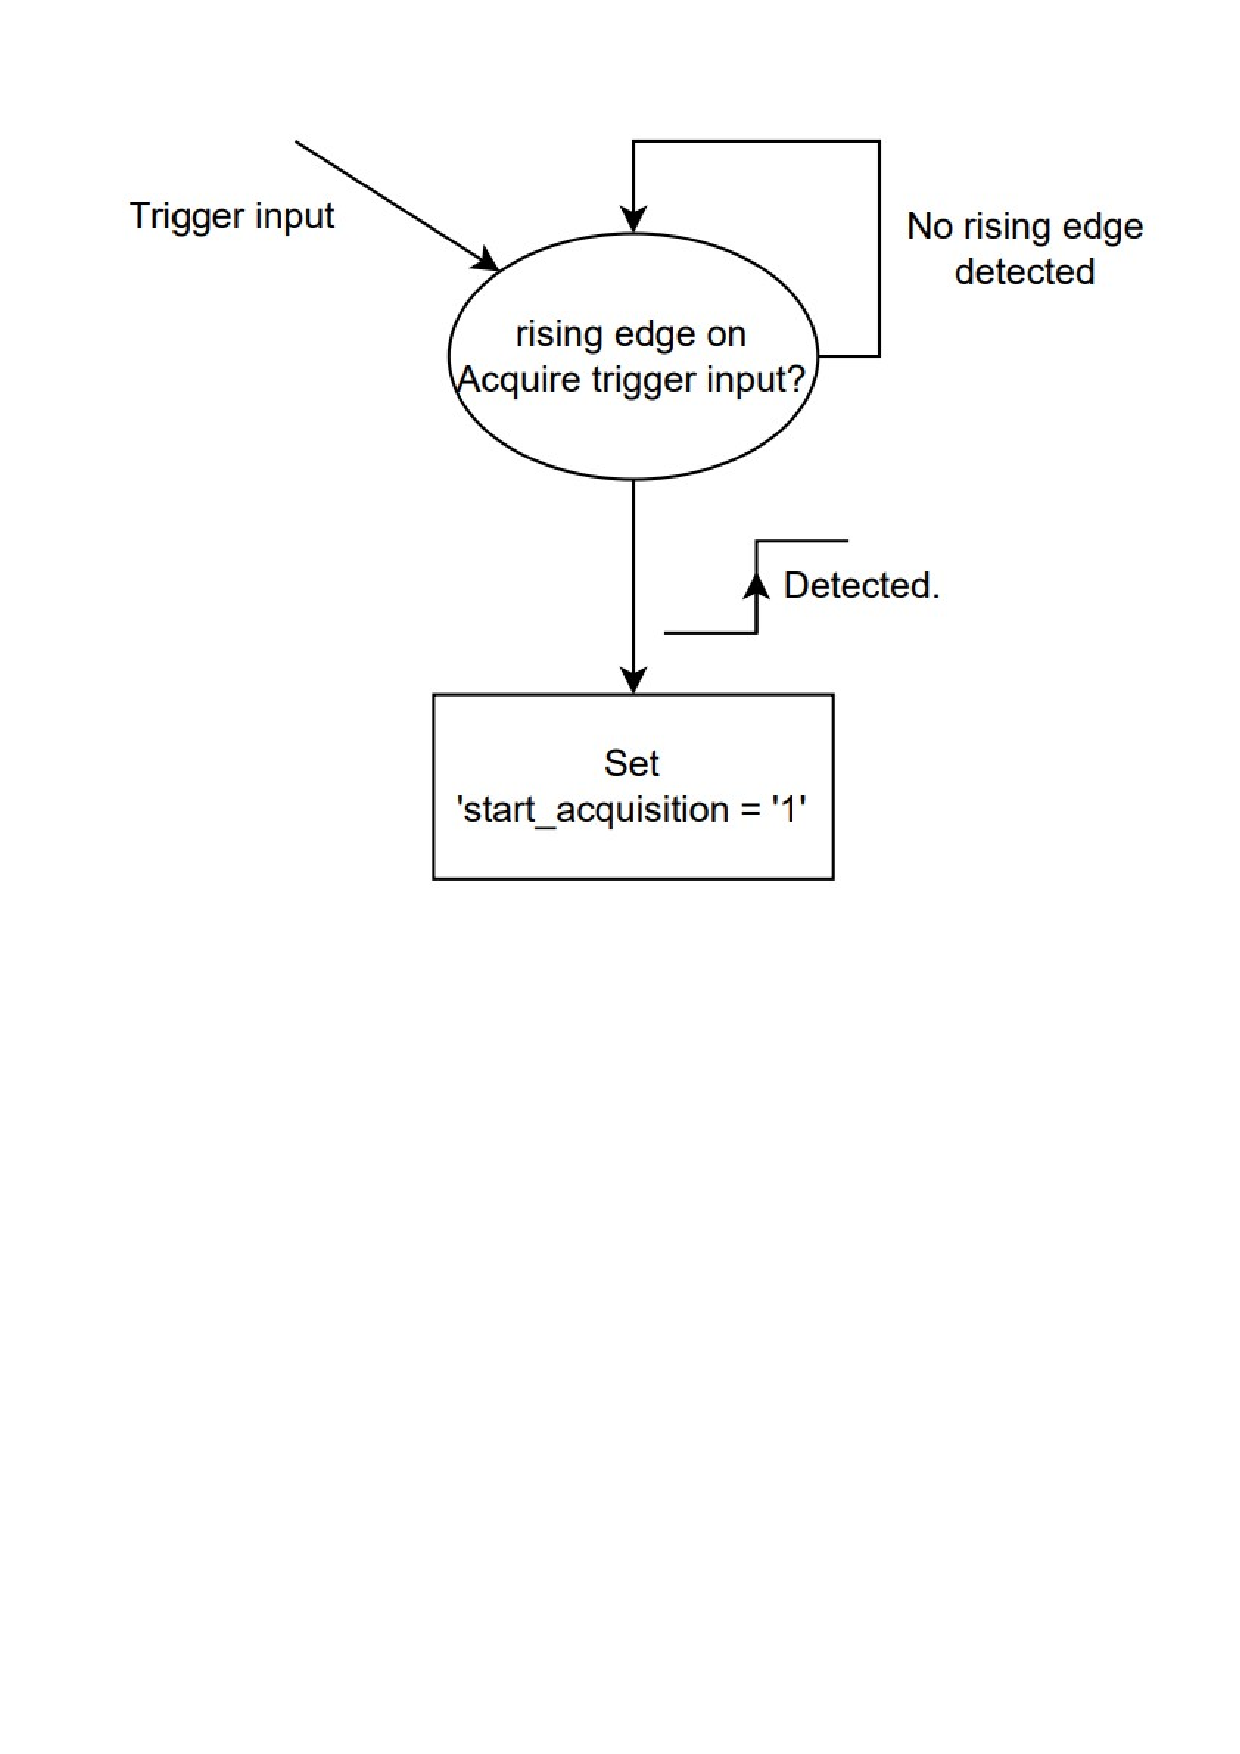
\includegraphics[clip, trim=0 300 0 0, width=0.5\textwidth]{Sections/7_SystemDesign/Figures/7_2_8_StartAcquisition.pdf}
    \caption{A trigger input will signal to the ADC control block that it should enable the FSM that controls the communication with the ADC.}
    \label{fig:7_2_8_ADC_START_ACQ}
\end{figure}

The "start\_acquisition" signal is checked in the FSM and will cause the FSM to start cycling through it's states, starting in the IDLE state and finishing in the LATCH state, as shown on figure \refq{fig:7_2_8_ADC_CONTROL_FSM}.

\begin{figure}[H]
    \centering
    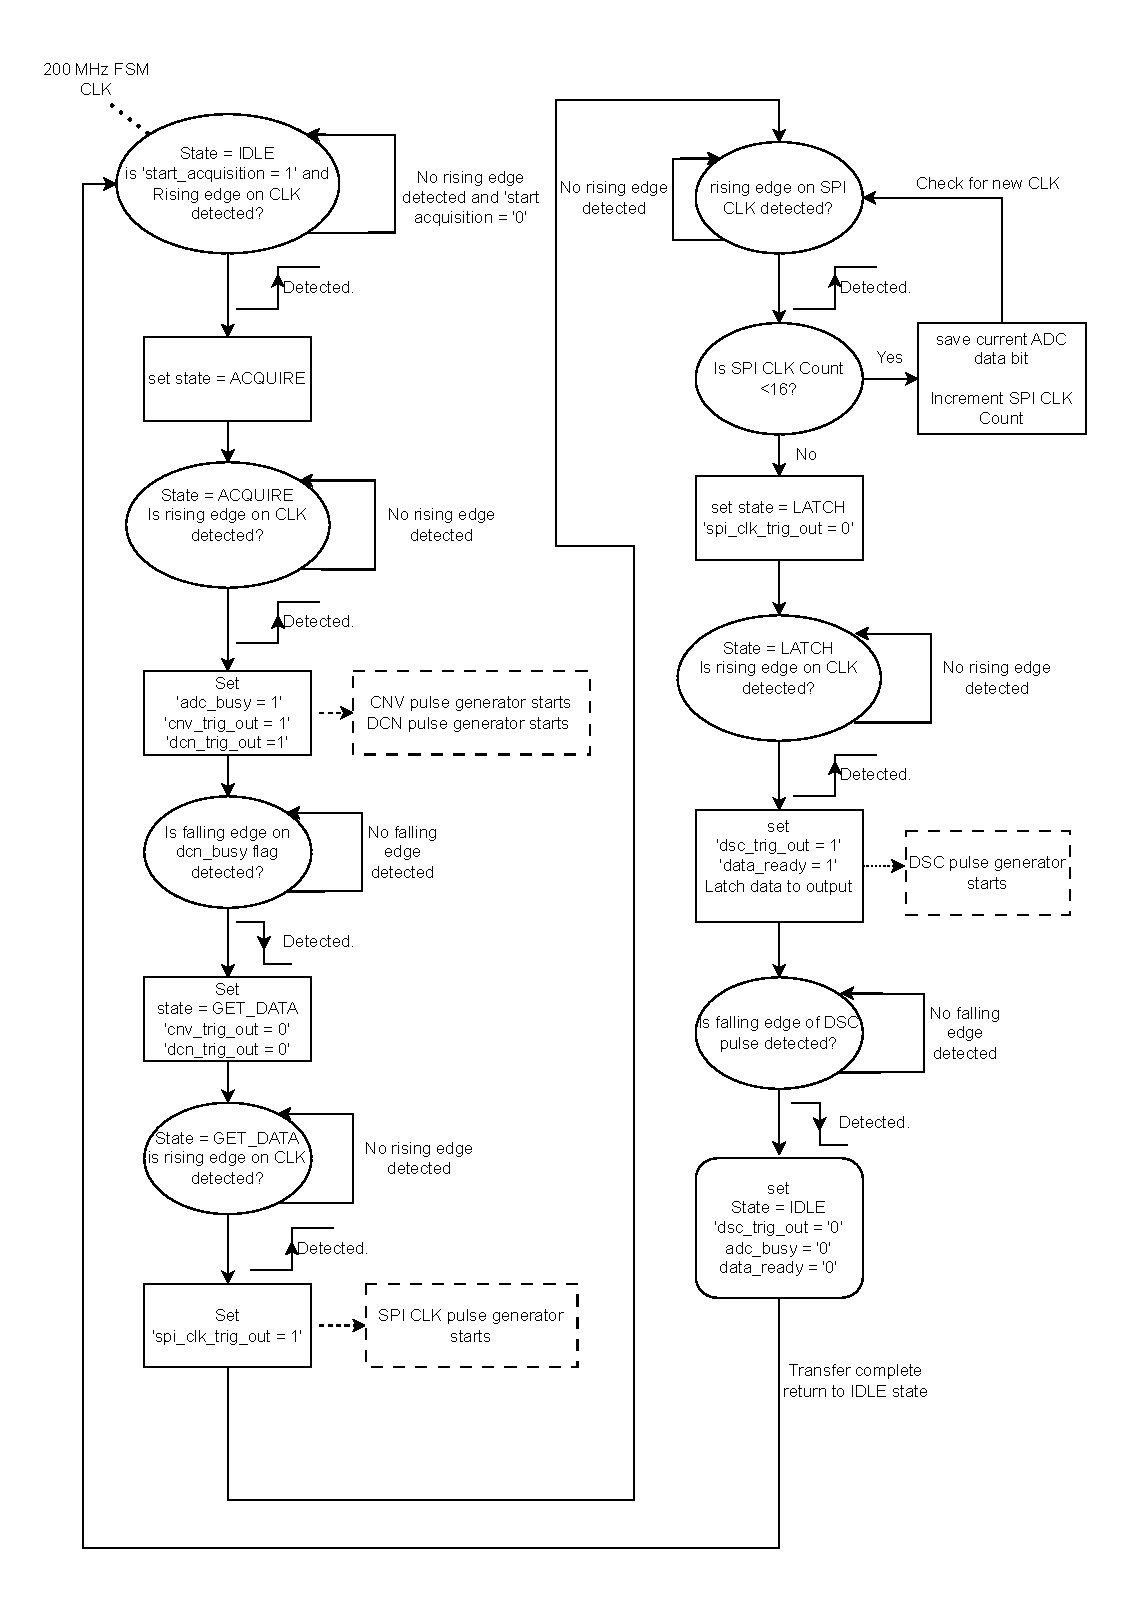
\includegraphics[clip, trim=0 0 0 0, width=0.9\textwidth]{Sections/7_SystemDesign/Figures/7_2_8_ADC Control Logic FSM.pdf}
    \caption{The state machine controlling the timing of the ADC. The FSM is clocked by a 200MHz clock and The FSM starts in the IDLE state in the upper left corner of the figure. The FSM will move from the IDLE state and down through the ACQUIRE and GET\_DATA states before it reaches the LATCH state where it will latch the data it has read from the ADC and return to the IDLE state. The data\_ready flag can be read by the next module in order to see when it should load the data from the ADC control module. The data should be read on a falling edge of the data\_ready flag. Note how the GET\_DATA and LATCH states will start some pulse generators that generate the CNV, DCN and DSC timing signals, these are marked in the dashed boxes. Each of these pulses have "busy" flags that are checked to see when those timing pulses have completed so the FSM can move on, in this way this FSM will generate the timing diagram shown on figure \refq{fig:7_2_8_LTC2311_TIMING}.}
    \label{fig:7_2_8_ADC_CONTROL_FSM}
\end{figure}

As shown on figure \refq{fig:7_2_8_ADC_CONTROL_FSM} the state machine has 4 states, namely IDLE, ACQUIRE, GET\_DATA and LATCH. In the IDLE state the FSM will wait for a trigger input from another module and remain inactive until this happens. When the start\_acquisition signal is asserted the FSM will switch to the ACQUIRE state and, on a rising edge of the master CLK signal, start both the CNV and DCN pulses shown on figure \refq{fig:7_2_8_LTC2311_TIMING}. A rising edge of the CNV pulse is what asserts the sample and hold circuit inside the LTC2311 ADC. The CNV and DCN pulse are generated by instantiations of the pulse generator shown in section \refq{subsec:Pulse_Generator}.

Note how on the timing diagram the DCN pulse is supposed to lag the CNV pulse, and not start at the point in time, this is done on purpose. The DCN pulse will start at the same time as the CNV pulse, but the pulse has the width of the sum of both $t_{CNV} + t_{DCN} = 45 ns$ and the result is that the SPI clock will start at the falling edge of the DCN pulse as desired.  

The various pulse generators used to generate the SPI CLK, CNV, DSC and CVN pulses interface with the ADC control block as shown on figure \refq{fig:7_2_8_PULSE_DELAY_TIMING} and the FSM diagram on figure \refq{fig:7_2_8_ADC_CONTROL_FSM}.

\begin{figure}[H]
    \centering
    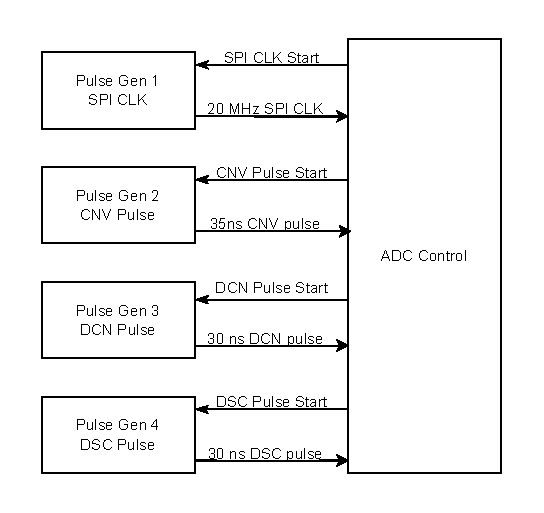
\includegraphics[clip, trim=0 15 0 0, width=0.5\textwidth]{Sections/7_SystemDesign/Figures/7_2_8_PulseAndADCControl.pdf}
    \caption{Various "pulse generators" are used to generate pulses, delays and clock signals in the ADC control module. The SPI CLK is of the type described in section \refq{subsec:PWMGen} and the CNV, DCN and DSC pulses are of the type described in section \refq{subsec:Pulse_Generator}.}
    \label{fig:7_2_8_PULSE_DELAY_TIMING}
\end{figure}

The GET\_DATA state shown on figure \refq{fig:7_2_8_ADC_CONTROL_FSM} will start the SPI CLK pulse generator. This pulse generator is a more advanced version of the pulse generator from section \refq{subsec:Pulse_Generator} and can control the high time and low time pulse widths. This pulse generator will be detailed in section \refq{subsec:PWMGen}. The pulse generator will generate 16 pulses, width a controlled width, that are used to CLK data out of the ADC and into the FPGA. On each falling edge of this CLK a bit is clocked out of the ADC and on the rising edge that same bit is clocked into the FPGA, starting with the MSb. The GET\_DATA state will save the data in a std\_logic\_vector and when it has counted 16 CLKs it will switch state to LATCH.

The LATCH state, will latch the data the FPGA has read when in the GET\_DATA state and signal the next module that it must read the data from the ADC control module. It generates a pulse on the data\_ready signal and data can be read on the falling edge of this signal. The reading module must latch the data before another AD-conversion finishes, or the data is overwritten and lost.

The timing of the ADC module has, of course, been simulated extensively, however it is difficult to show this in this document and the result will vary slightly depending on the actual implementation on the FPGA. The output of the ADC control module has also been verified by use of measurements in order to ensure the correct timing after implementation. A measurement of the acquisition start CNV pulse can be seen on figure \refq{fig:7_2_8_ADC_CONTROL_CNV_MEAS} where the width of the pulse is exactly \SIQ{35}{\nano\second} as expected. 

\begin{figure}[H]
    \centering
    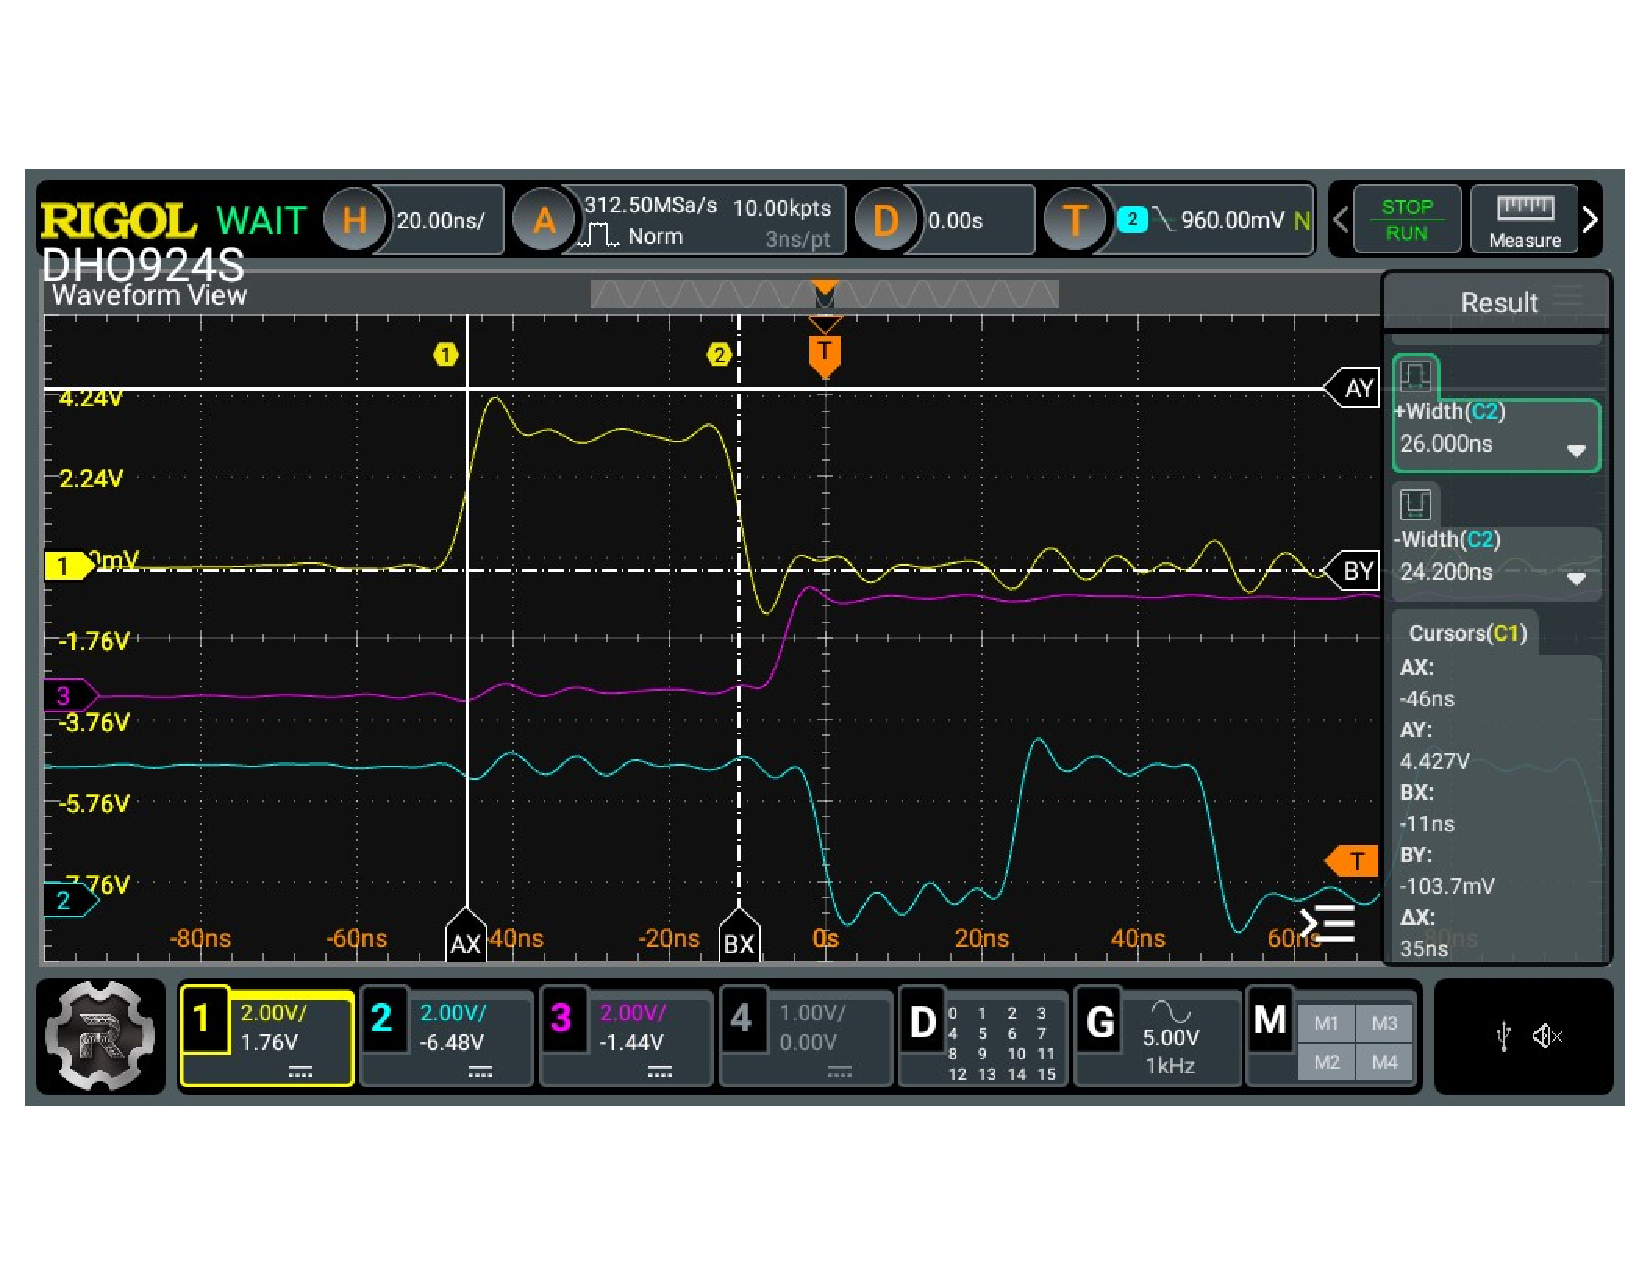
\includegraphics[clip, trim=0 100 0 0, width=0.9\textwidth]{Sections/7_SystemDesign/Figures/7_2_8_ADCControl_CNV_MEASURE.pdf}
    \caption{A measurement of the CNV pulse width. The yellow trace is the CNV pulse. The width is $\Delta X = 35 ns$ as shown in measurement window on the right side of the screen.}
    \label{fig:7_2_8_ADC_CONTROL_CNV_MEAS}
\end{figure}

The DCN time, or, the delay between the falling edge of the CNV pulse and the first falling edge of the SPI CLK signal must be atleast \SIQ{9.5}{\nano\second}, this has also been verified and can be seen on figure \refq{fig:7_2_8_ADC_CONTROL_DCN_MEAS}.

\begin{figure}[H]
    \centering
    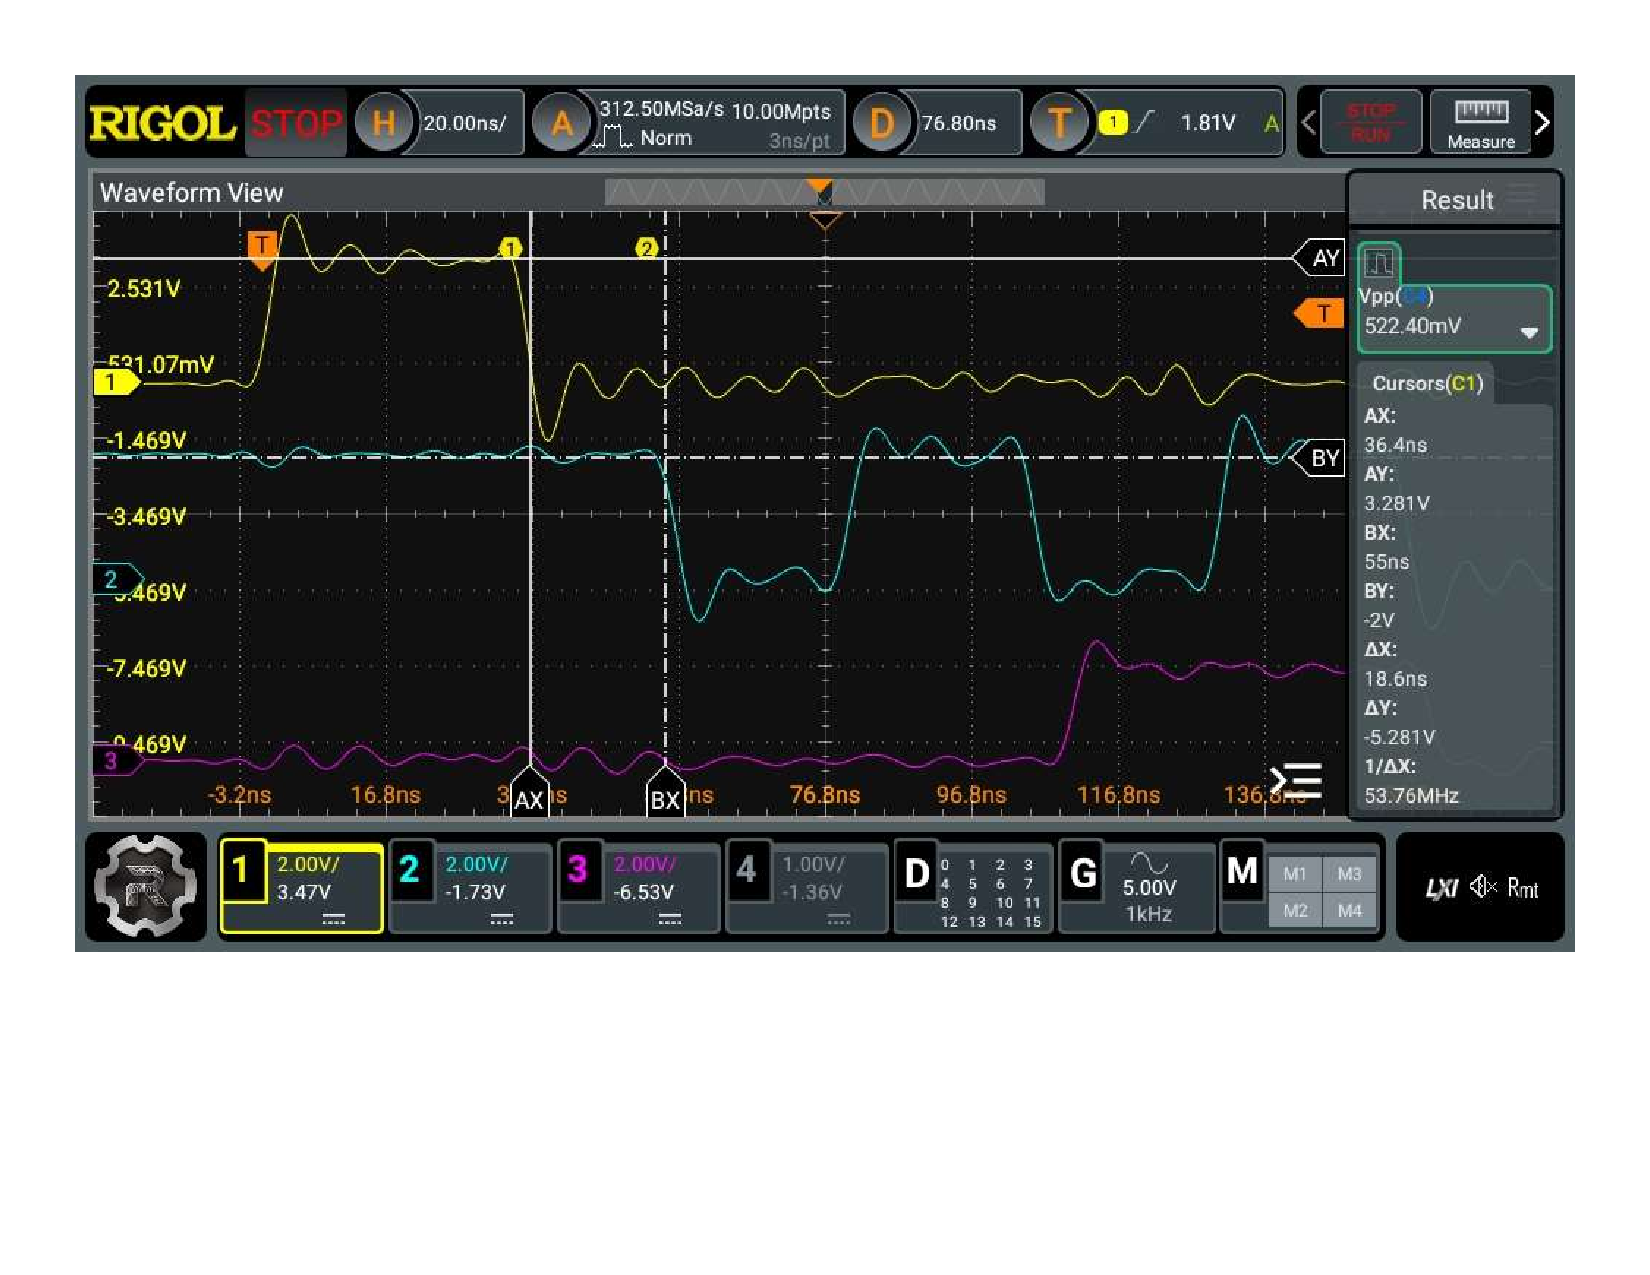
\includegraphics[clip, trim=0 150 0 0, width=0.9\textwidth]{Sections/7_SystemDesign/Figures/7_2_8_ADC_CONTROL_DCN_MEAS.pdf}
    \caption{A measurement of the DCN pulse width. The yellow trace is the CNV pulse and the blue trace is the SPI CLK signal. The delay between the falling edge of CNV and falling edge of SPI CLK is $\Delta X = 18.6 ns$ as shown in measurement window on the right side of the screen.}
    \label{fig:7_2_8_ADC_CONTROL_DCN_MEAS}
\end{figure}

The DCN time is slightly longer than the expected \SIQ{15}{ns} due to the actual implementation, but this is OK, a shorter time would not be OK. The SPI CLK frequency has also been verified and can be seen on figure \refq{fig:7_2_8_ADC_CONTROL_SPI_CLK}

\begin{figure}[H]
    \centering
    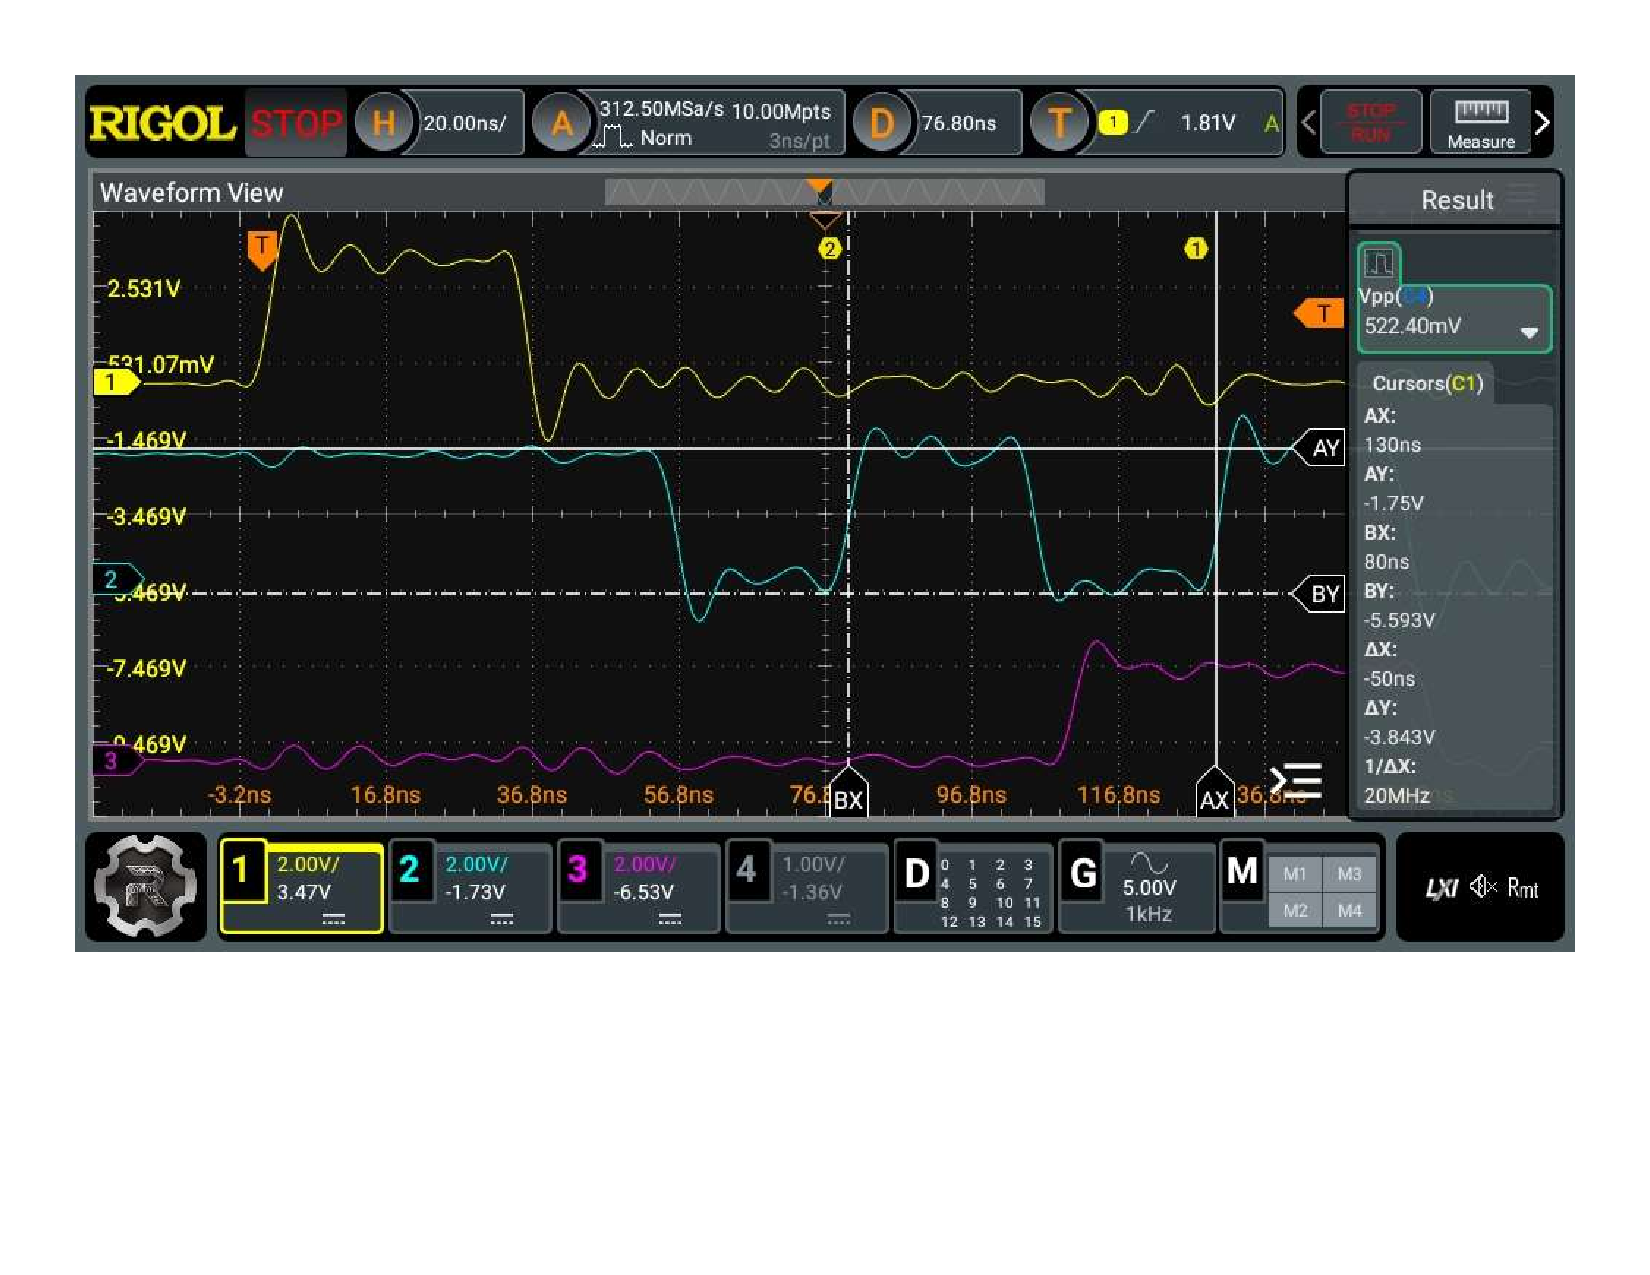
\includegraphics[clip, trim=0 150 0 0, width=0.9\textwidth]{Sections/7_SystemDesign/Figures/7_2_8_ADC_CONTROL_SPICLK.pdf}
    \caption{A measurement of the SPI CLK frequency. The CLK frequency is 20MHz as shown in the right side of the screen.}
    \label{fig:7_2_8_ADC_CONTROL_SPI_CLK}
\end{figure}

The DSC time has not been verified by measurement, only simulation, instead it has been verified that the ADC control will function at a sample rate of, at least, 1MS/s as was the goal for the module. Several consequtive ADC acquisitions and data transfers can be seen on figure \refq{fig:7_2_8_ADC_CONTROL_1MEGASAMPLE} which proves that the module will work at the desired sample rate as there is no corruption of the communication signals.

\begin{figure}[H]
    \centering
    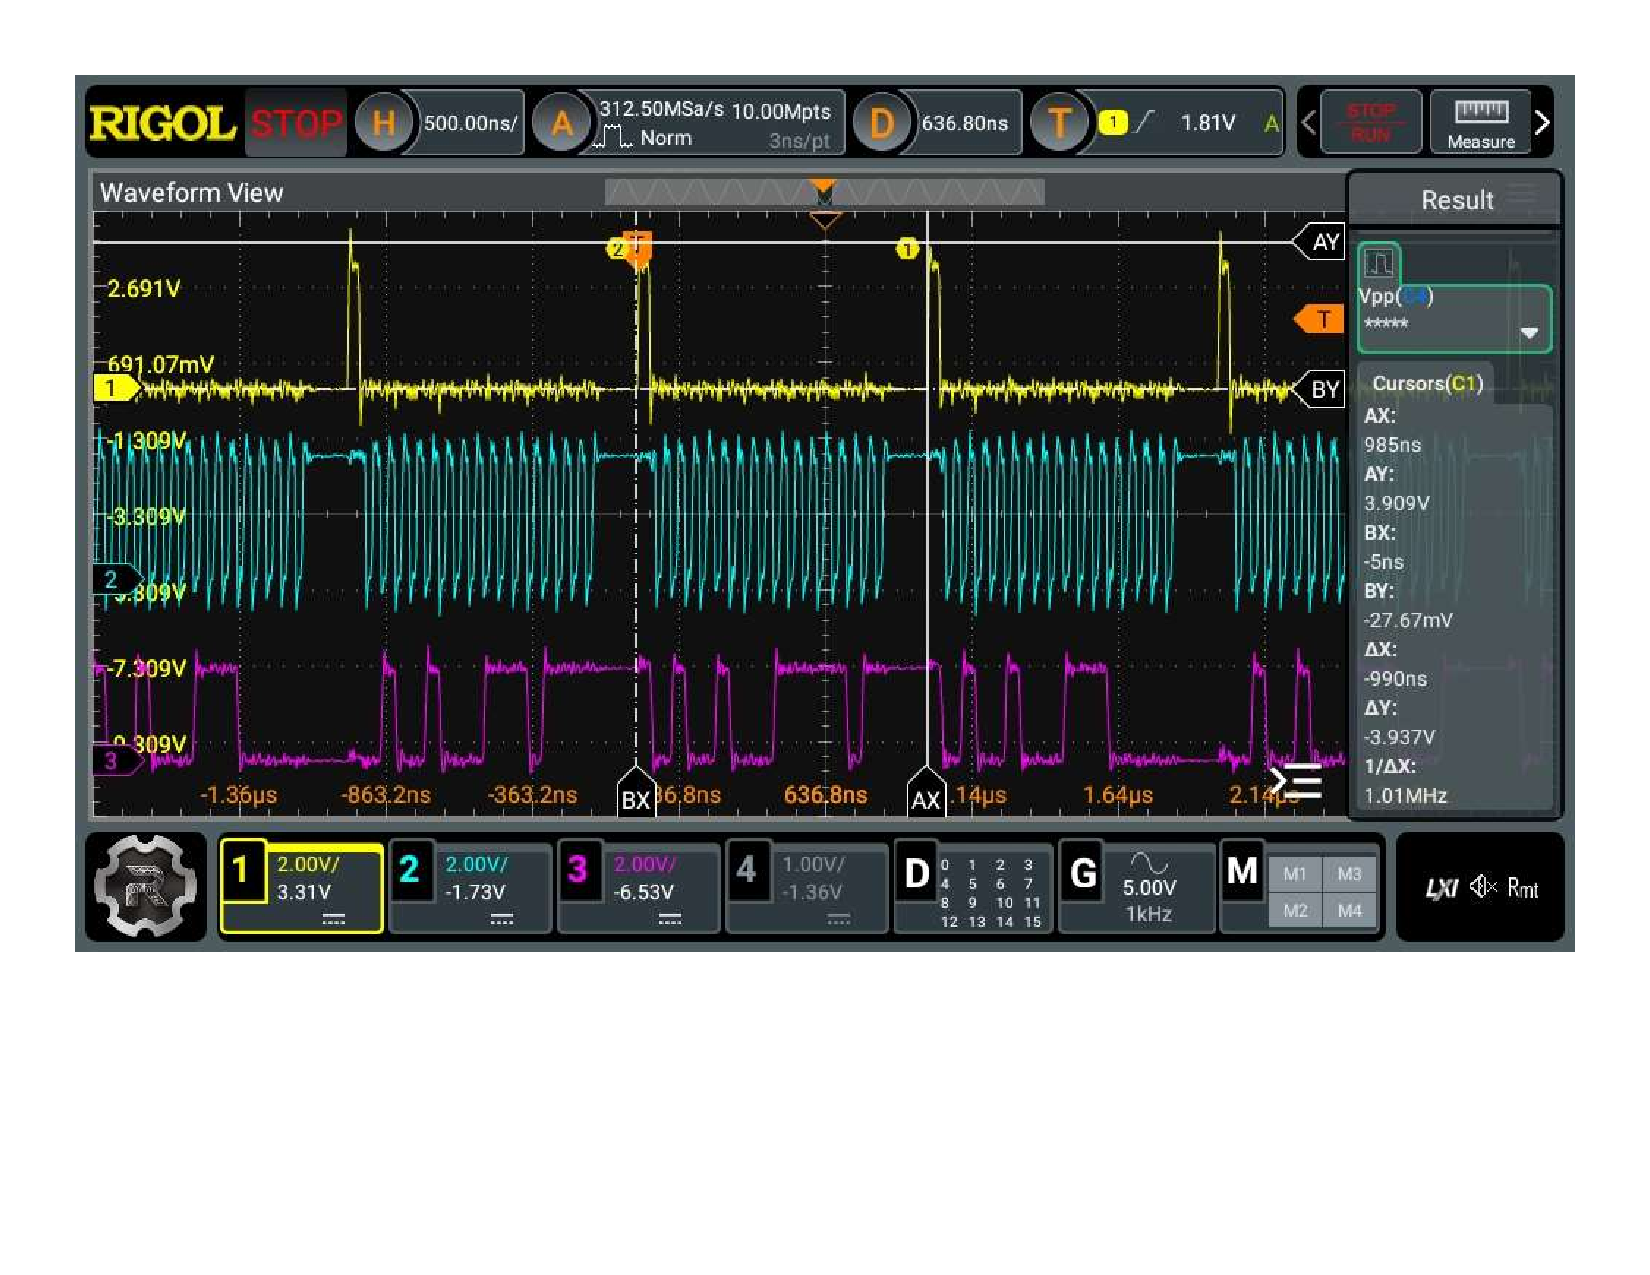
\includegraphics[clip, trim=0 150 0 0, width=0.9\textwidth]{Sections/7_SystemDesign/Figures/7_2_8_ADC_CONTROL_1MEGSAMPLE_MEAS.pdf}
    \caption{Several consequtive AD-conversions and data transfers. The ADC control module is working as expected at 1 MS/s. The time between the acquisitions can be seen in the right hand side of the screen which shows the frequency of the CNV pulse, and thus sample rate, is 1 MHz.}
    \label{fig:7_2_8_ADC_CONTROL_1MEGASAMPLE}
\end{figure}

As can be seen on figure \refq{fig:7_2_8_ADC_CONTROL_1MEGASAMPLE} the ADC control hardware will work at 1MS/s. There is even time to spare before the next cycle begins. The module can easily be modified to run higher sample rates by adjusting the pulse generators being used in this module, though it may require the use of differential clock and data lines between the FPGA and LTC2311 ADC. The test setup for these measurements, and the measurements themselves can be found in appendix \refq{App:ADCControlMeasurement}.
